\documentclass[12pt, oneside]{article} 
\usepackage[left=15mm, right=15mm, top=10mm]{geometry}
\usepackage{graphicx}
\usepackage{url}
\usepackage{multicol}
\usepackage{hyperref}
\usepackage{float}

\begin{document}
\title{Techniques d'attaque - attaques DoS et botnets}
\author{Tristan BILOT, Nora DELFAU, Enzar SALEMI, Madushan THAMBITHURAI\\EPITA}
\date{8 Juin 2021}
\maketitle

\begin{abstract}
L'objectif de ce cours est d'apprendre les bases concernant les attaques par déni de service et leur utilisation par des botnets. Les différentes méthodes d'attaque DoS seront utilisées, notamment l'attaque DDoS.
\end{abstract}

\section{Notes}
\subsection{DoS \& DDoS}

\begin{itemize}
\item DoS: une attaque DoS (attaque par déni de service) est une attaque  dans laquelle l'auteur cherche à rendre une machine ou une ressource réseau indisponible pour ses utilisateurs prévus en perturbant temporairement ou indéfiniment les services d'un hôte connecté à Internet.

\item DDoS: Distributed Denial Of Service. L'objectif est d'utiliser la puissance de plusieurs machines afin d'inonder la machine cible. Si l'ensemble de nos machines est plus puissant que la machine attaquée, alors l'attaque sera capable d'empêcher son fonctionnement si aucune action contre cette technique n'est mise en place.
\end{itemize}

\begin{itemize}
\item Par inondation: l'attaque DoS la plus courante. Le concept est d'envoyer plus de trafic vers une adresse réseau que ce que les développeurs ont construit pour gérer le système.

\item Par exploitation d'une vulnérabilité: d'autres attaques DoS exploitent simplement les vulnérabilités qui provoquent le plantage du système ou du service cible. Dans ces attaques, une input est envoyée qui tire parti des bugs dans la cible qui par la suite plantent ou déstabilisent gravement le système, de sorte qu'il ne peut pas être consulté ou utilisé.
\end{itemize}

\subsubsection{Techniques DoS}
\begin{itemize}
\item Ping of death: à l'époque, le protocole IP ne gérait pas le cas ou le paquet ping passant par le protocole ICMP. Envoyer un paquet ICMP contenant trop de data sera alors interprété par une erreur côté serveur.
\item IP spoofing: ceci n'est pas une technique d'attaque mais une technique utilisée pour de la dissimulation: on change de façon aléatoire l'adresse IP source afin d'éviter de se faire détecter. Toutefois, ce n'est pas suffisant pour ne pas détecter un DDoS.
\item Land attack: lors de l'envoi d'un paquet, la destination et la source sont l'adresse de la victime, ce qui mettra en place une sorte de boucle, créant un déni de service. Patché aujourd'hui mais toujours présent sur certaines implémentations.
\item Teardrop: Chaque protocole de communication réseau possède un MTU: la taille maximale d'un paquet fragmenté. Dans le protocole IP, dans le cas où il manque un fragment à un paquet, le paquet est annulé. L'objectif de cette attaque vise alors à supprimer un fragment et ainsi empêcher l'envoi du paquet en entier. Cela permet donc de bloquer l'envoi de paquets.
\item Black hole: c'est un type d'attaque dans laquelle un routeur censé relayer les paquets les rejette. Cela se produit généralement lorsqu'un routeur est compromis pour un certain nombre de causes différentes. Une cause mentionnée dans la recherche est une attaque par déni de service sur le routeur à l'aide d'un outil DDoS connu.
\item TCP SYN flood: Dans le protocole TCP: le handshake s'effectue en 3 étapes, envoi d'un SYN au serveur, réponse SYN/ACK du serveur puis envoi d'un ACK au serveur. Le serveur alloue un espace mémoire pour chaque réception d'un SYN. L'objectif de cette attaque est d'envoyer massivement des SYN mais sans ACK afin que la stack du serveur créé un overflow. Pour s'en prémunir, les serveurs vont attendre une très courte période entre l'envoi du SYN/ACK et la réponse ACK puis libérer la mémoire. Grâce à cela, il sera compliquer d'envoyer suffisamment de paquets en une très courte période afin d'exploiter cette vulnérabilité. Toutefois, elle reste l'une des attaques les plus utilisées et est un succès dans le cas ou on possède une grande puissance d'envoi de paquets.
\begin{figure}[H]
\centering
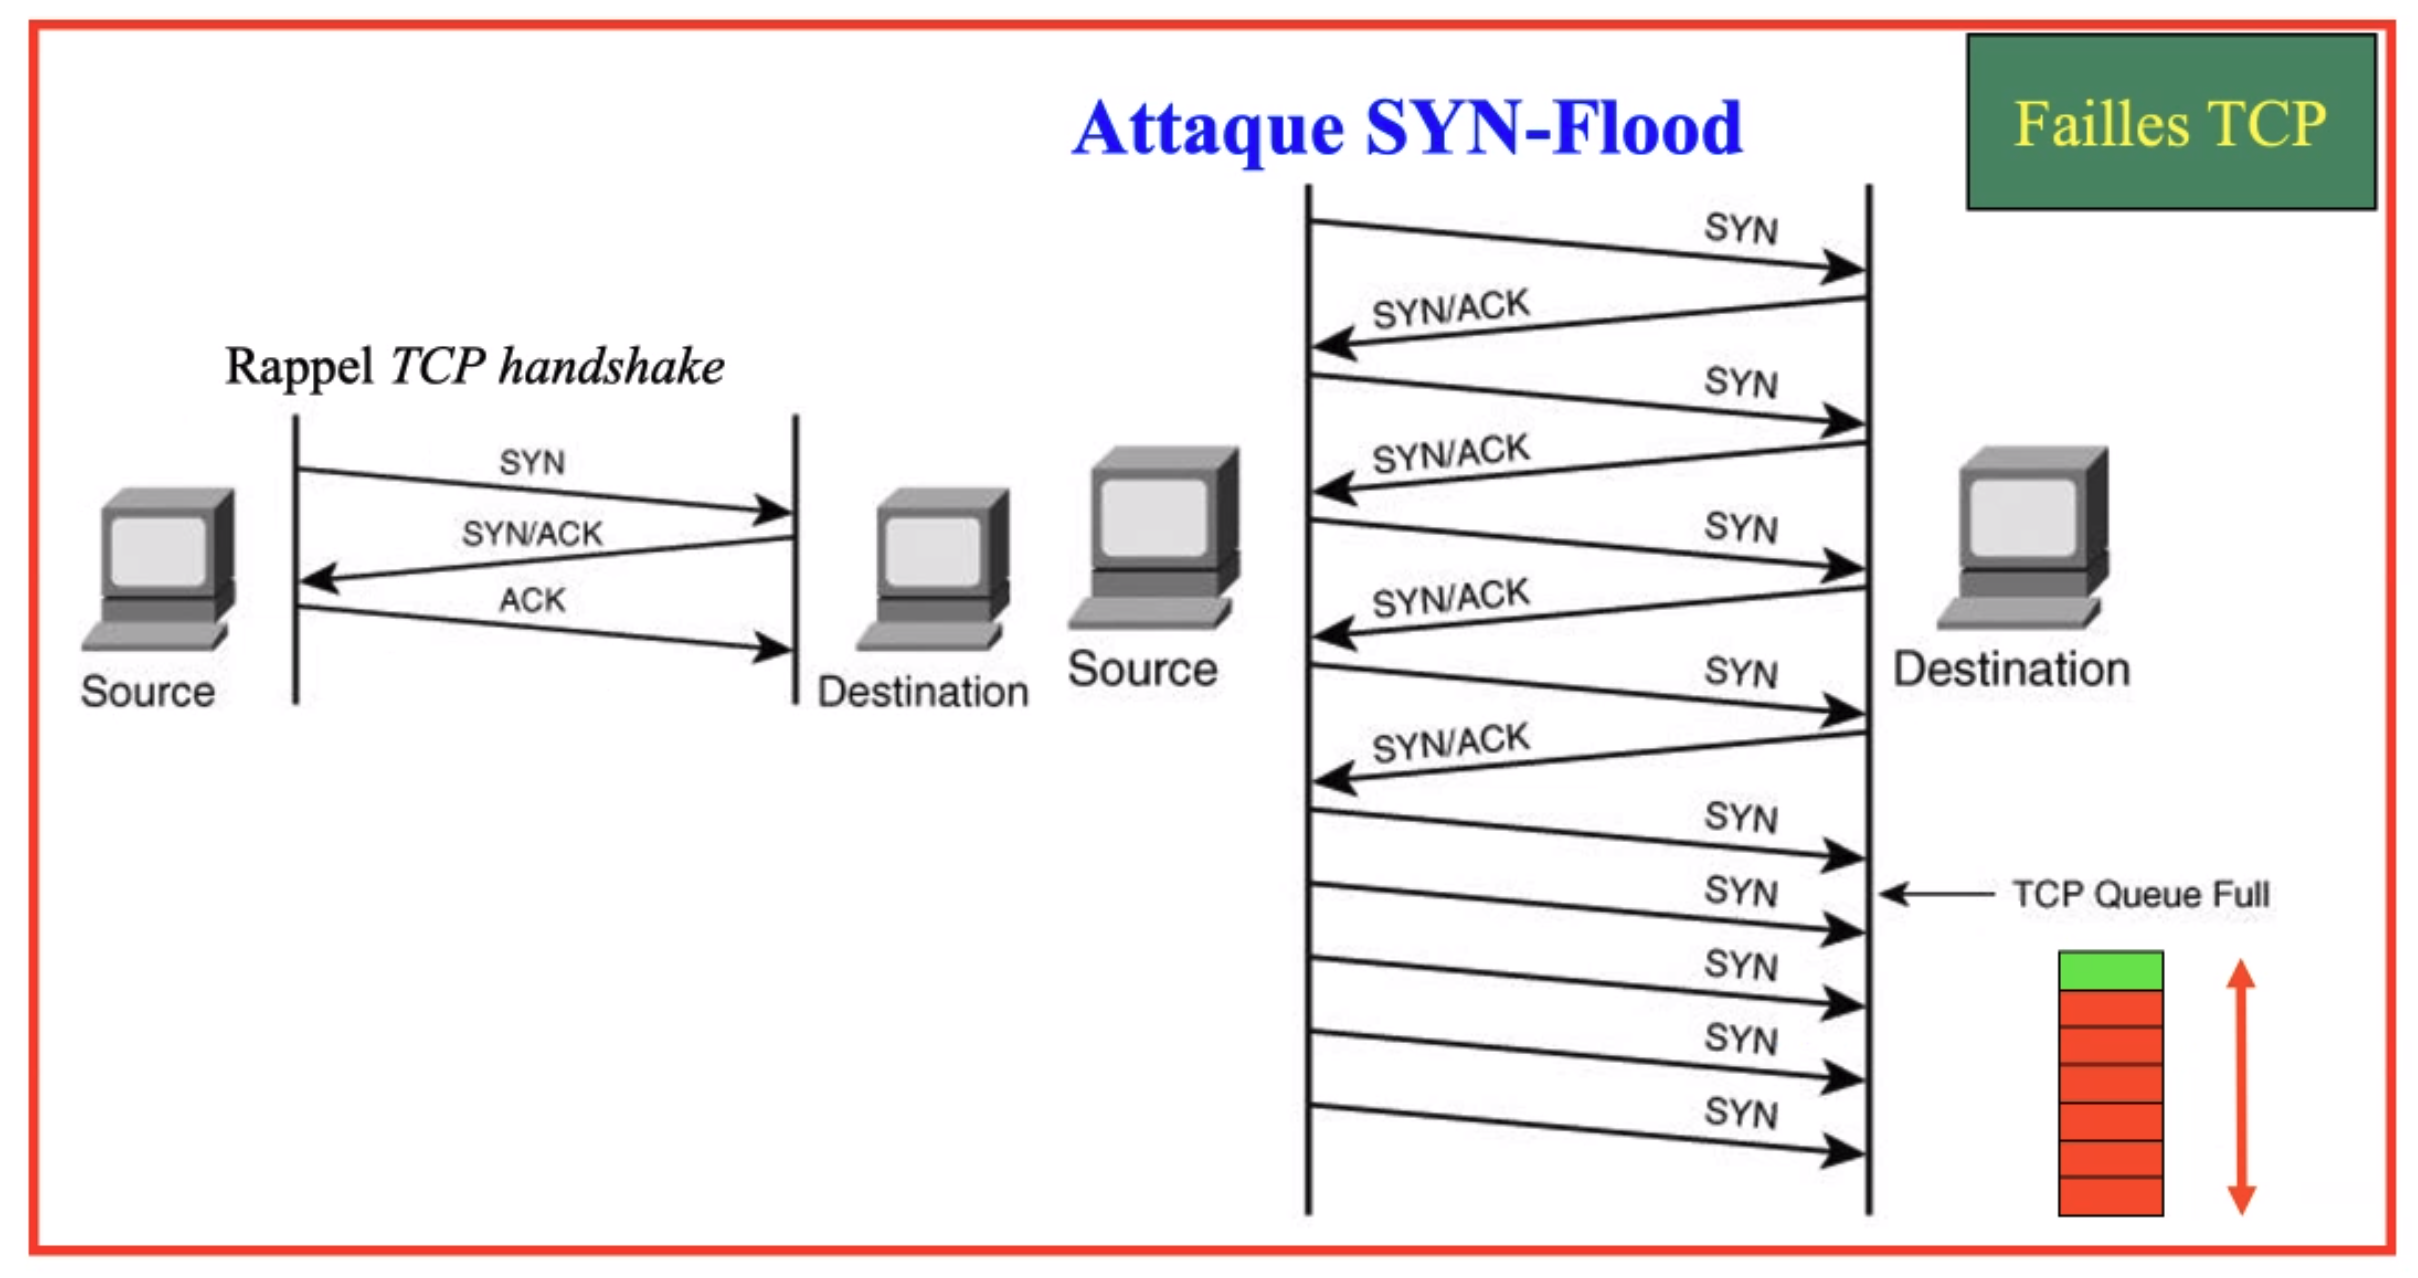
\includegraphics[scale=0.4]{syn-flood}
\caption{Attaque SYN-Flood}
\end{figure}
\item UDP flood: chaque routeur est capable de handle une certaine quantité d'octets par seconde, si le nombre de requêtes est supérieur à ce que peut supporter le routeur, une file d'attente est créé afin que les dernières personnes ayant envoyé une requête attendent la fin de la file d'attente. L'objectif de cette attaque est de flooder le routeur afin d'augmenter le temps d'attente des requêtes. La plupart des entreprises refusent d'accepter de l'ICMP donc aujourd'hui on utilise de l'UDP.
\begin{figure}[H]
\centering
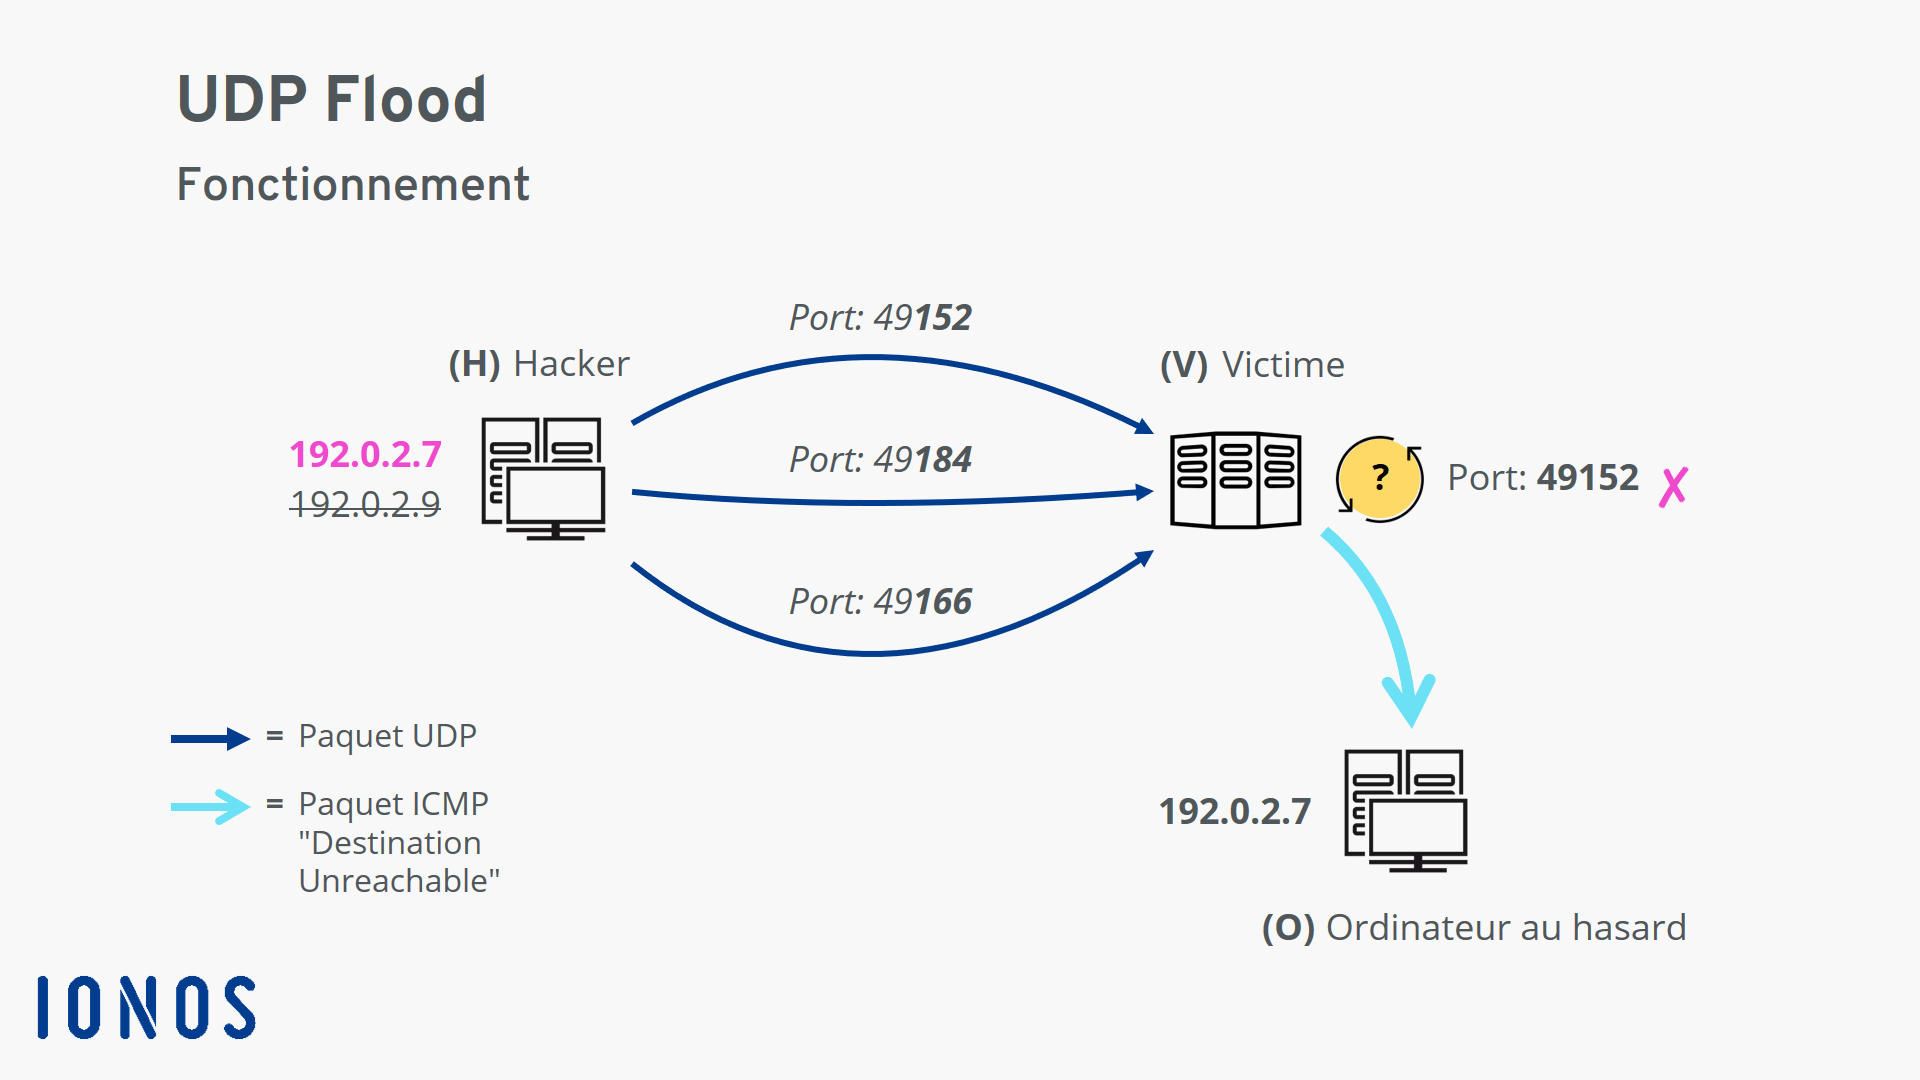
\includegraphics[scale=0.23]{udp-flood}
\caption{Attaque UDP flood}
\end{figure}
\item Reflective attack/Smurf: l'objectif de l'attaque est d'envoyé un nombre important de requête avec IP source la victime. Ainsi les réponses aux requêtes seront renvoyées à la victime, créant un déni de service.
\begin{figure}[H]
\centering
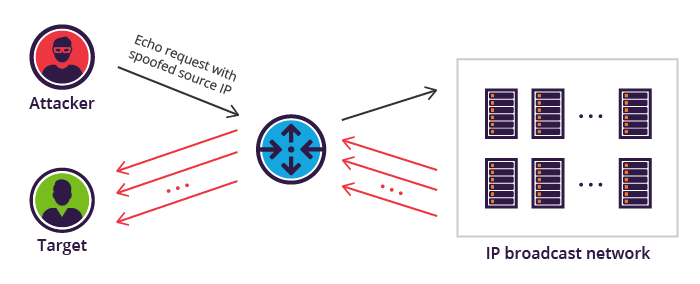
\includegraphics[scale=0.23]{smurf}
\caption{Attaque Smurf}
\end{figure}
\item Amplification attack: reflective attack mais avec une réponse beaucoup plus grande. Exemple: dns reflection => le serveur dns renvoie une table de translation potentiellement très grande (plusieurs Mo). On envoie des requêtes à des serveurs DNS avec comme adresse IP source l'IP de la victime donc la victime s retrouve avec un flux immense de données à handle. Cette attaque est utilisable dans le cas ou on possède un botnet contenant un grand nombre de machines qui enverront des requêtes aux serveurs DNS (environ 32 millions de serveurs DNS sur Internet dont 28 millions accessibles librement). Pays-bas en 2013, une attaque de ce type a été effectuée et le réseau du pays a été down.
\item NTP reflection: Network Time Protocol: utilisé pour ordonnancer le flux sur les réseaux. Les serveurs RTP vont répondre les 600 dernières adresses IP avec lesquelles ils ont communiqués et on peut exploiter ces réponses pour une attaque DoS.\\
\end{itemize}
\subsubsection{Informations générales}
En 2018 la plus grande attaque DDoS était d'un débit de 1,7Tb/s et en 2020: 2,5Tb/s.
La majorité des attaques DDoS est inférieur à 4h. On compte 10\% des attaques entre 4 et 8h. C'est très rare de trouver des attaques plus longues. Dans le cas où un load balancer est utilisé côté défense, il va dispatcher les requêtes mais risque d'être down si l'attaque est trop grosse. La Chine en 2019 concentre 68\% des attaques DDoS. On estime qu'environ 45\% des machines en Chine sont infectées et font partie de botnets. Pourquoi la Chine? Car le pays contient énormément de petites entreprises contenant des réseaux non sécurisés et donc vulnérables.

\subsection{Botnet}
Botnet: collection/réseau d'ordinateurs compromis qui sont utilisés à l'insu de leurs utilisateurs afin d'utiliser des attaques. (Bot: robot, Net: network). Le botmaster est la personne manageant ce réseau. Le serveur C\&C: command and control server est la machine maître qui va contrôler le réseau et envoyer les commandes.

\subsubsection{Botnet centralisé}
Dans les botnets centralisés simples, on aura le botmaster qui sera également le C\&C. Sinon dans des botnets centralisés évolués, on aura plusieurs niveaux de C\&C contrôlés par un botmaster. Les machines infectées communiquent avec les C\&C et non le botmaster directement afin de ne pas retrouver le botmaster. En revanche si un C\&C est down, toutes les machines infectées ne pourront plus communiquer avec.
\begin{figure}[H]
\centering
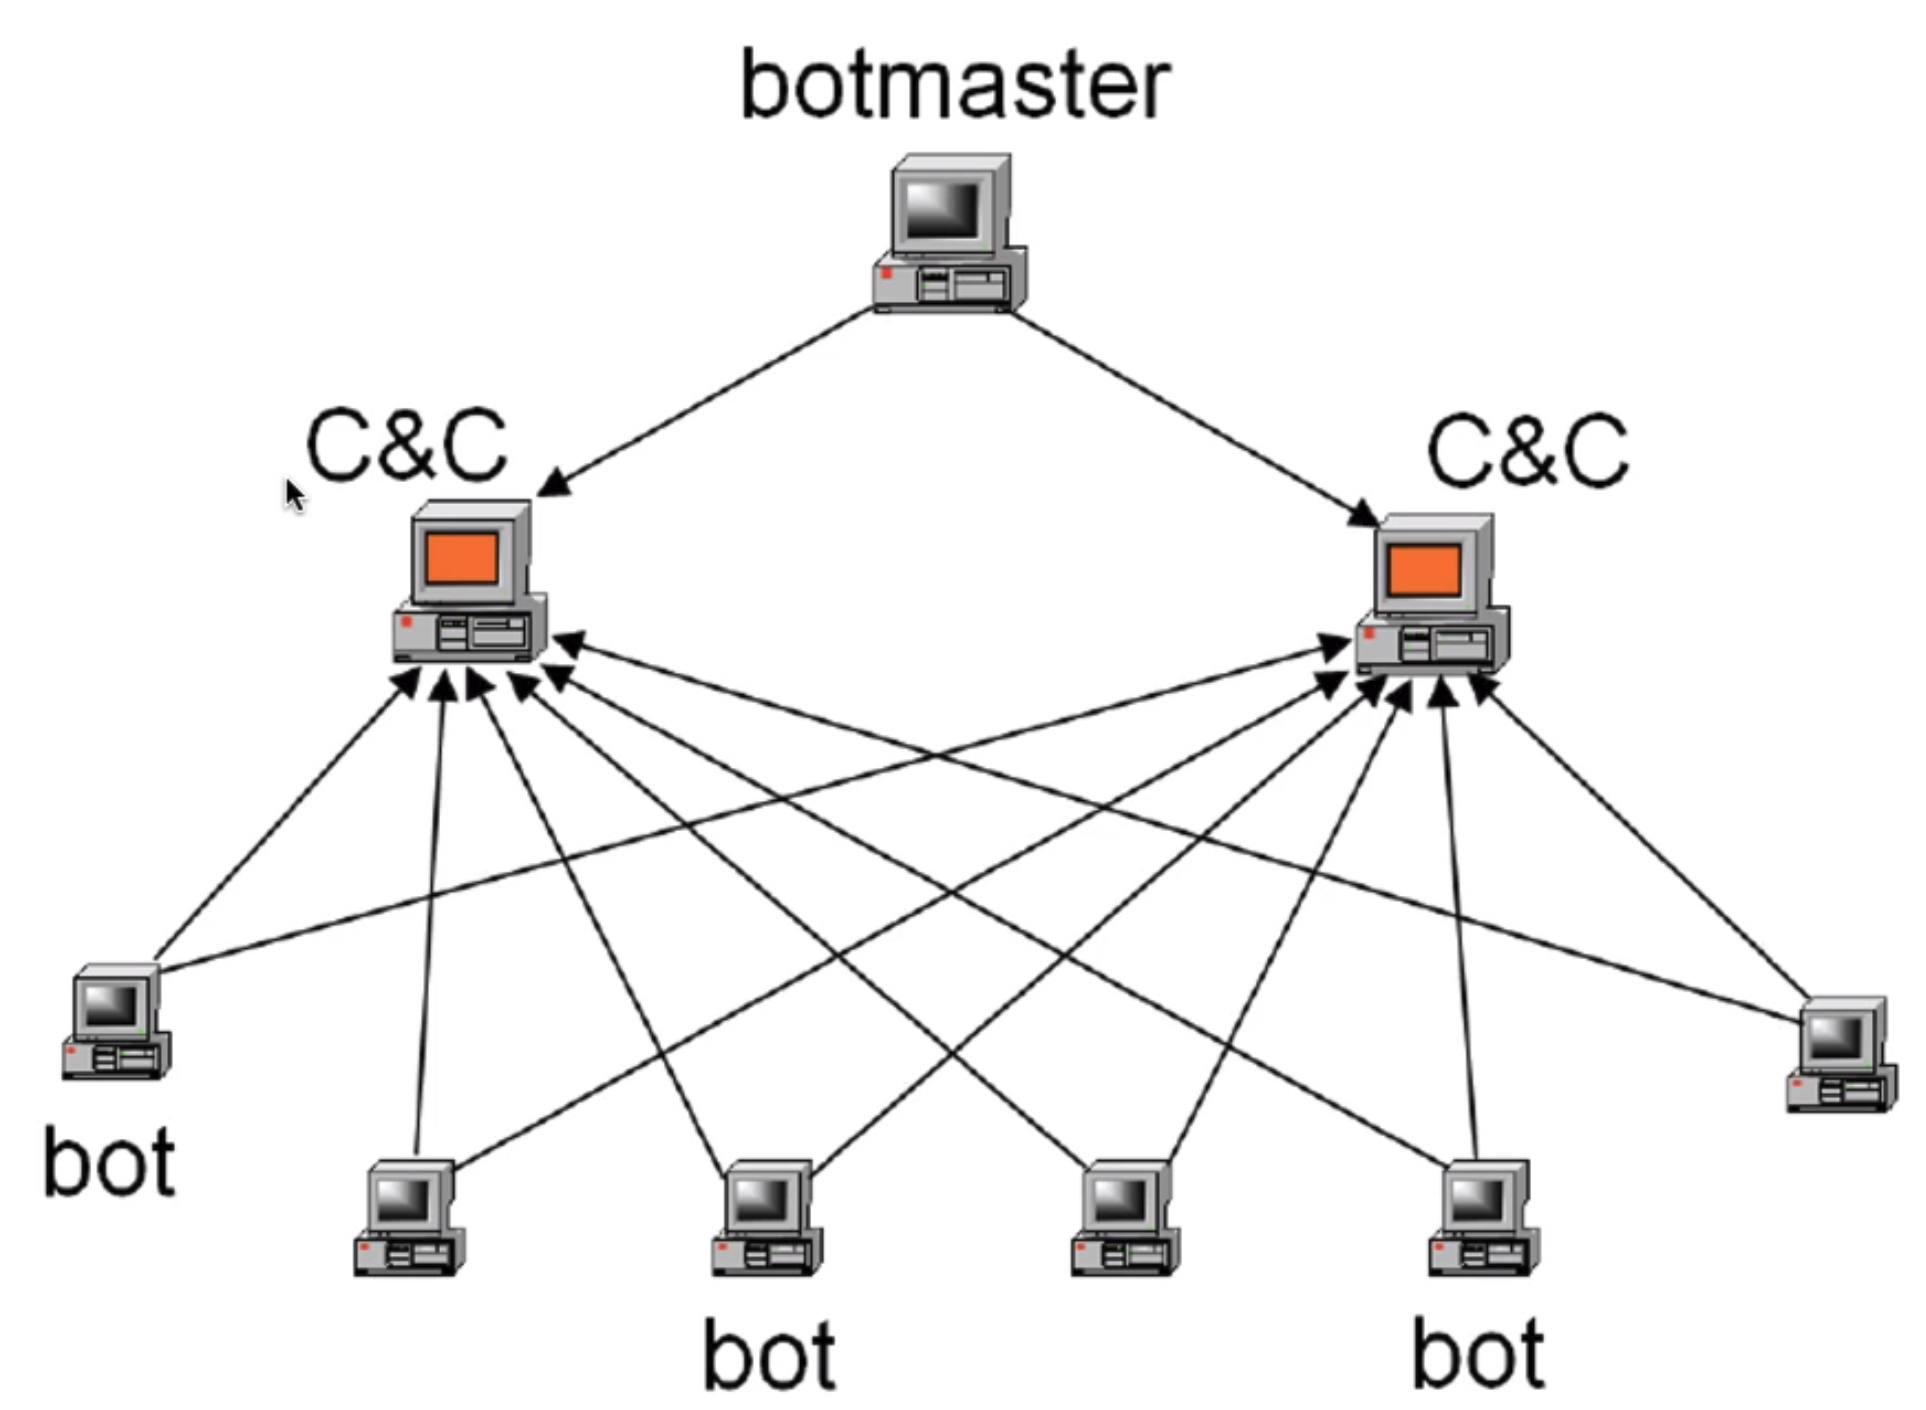
\includegraphics[scale=0.3]{centralized}
\caption{Architecture d'un botnet centralisé}
\end{figure}

\subsubsection{Botnet décentralisé}
Contrairement au mode centralisé, le réseau fonctionne en peer-to-peer et donc en mettant down une machine, cela n'affecte pas le réseau. En revanche, la communication n'étant plus centralisé il devient donc plus compliqué aux machines de communiquer au sein du réseau.
\begin{figure}[H]
\centering
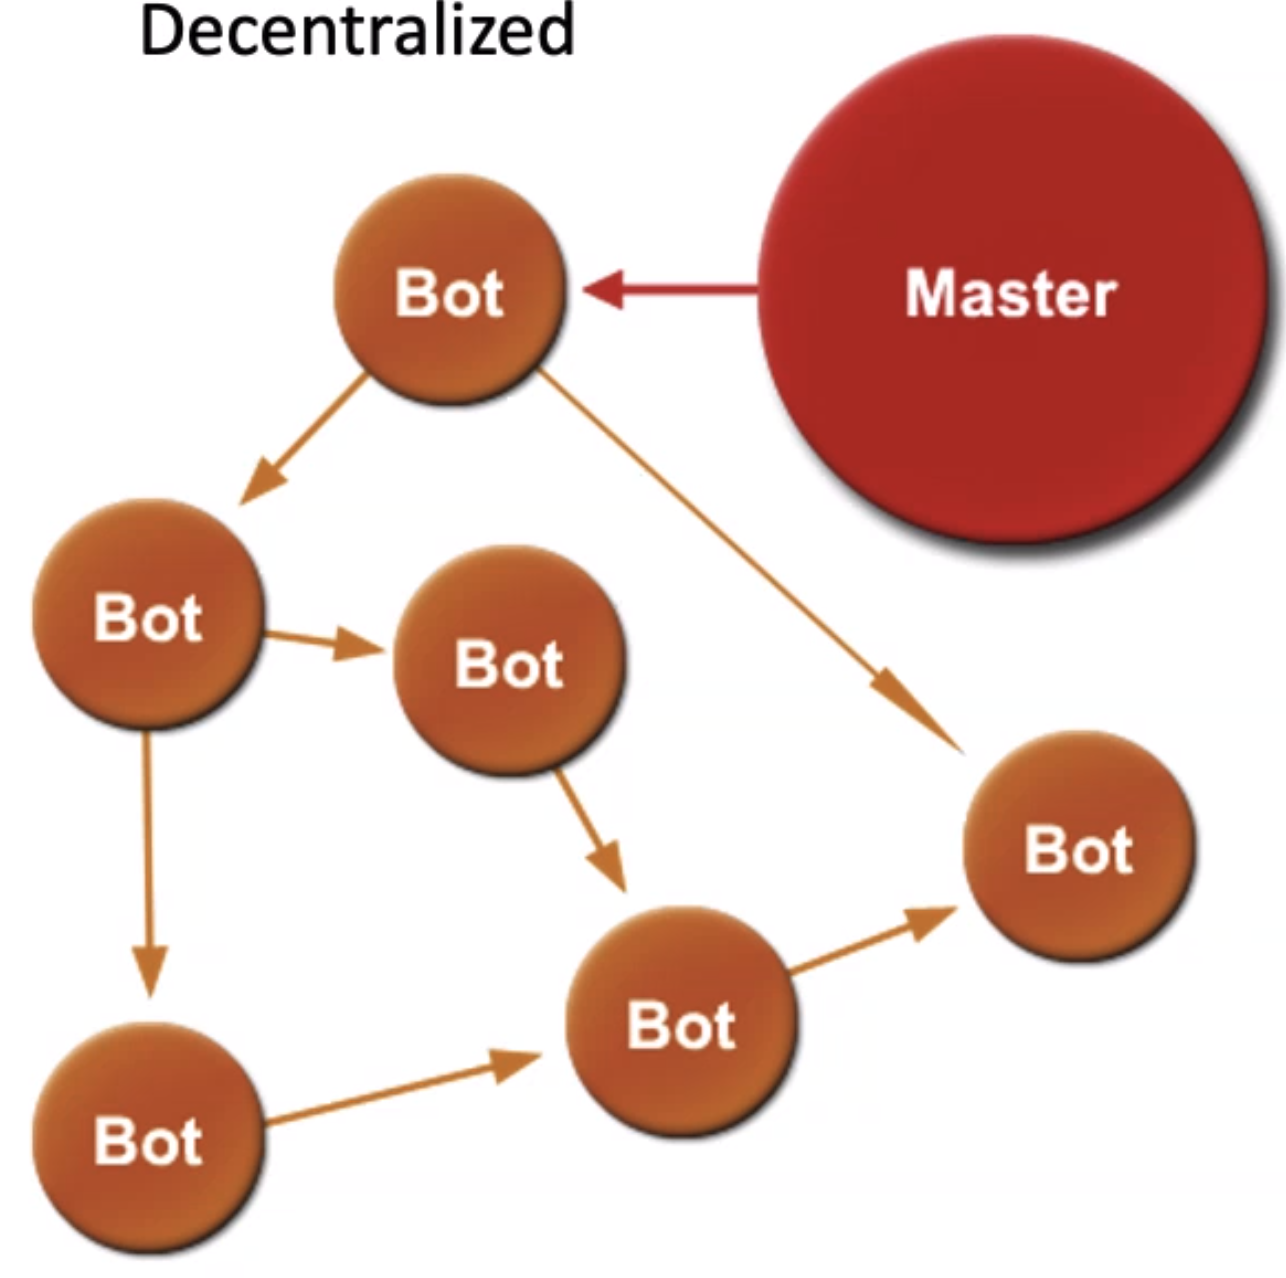
\includegraphics[scale=0.3]{decentralized}
\caption{Architecture d'un botnet décentralisé}
\end{figure}

\subsubsection{Botnet hybride}
Ce type de botnet mélange les 2 techniques. Pour plus de détails sur le fonctionnement, voir \href{https://www.usenix.org/legacy/event/hotbots07/tech/full_papers/wang/wang_html/}{ce papier}.
\begin{figure}[H]
\centering
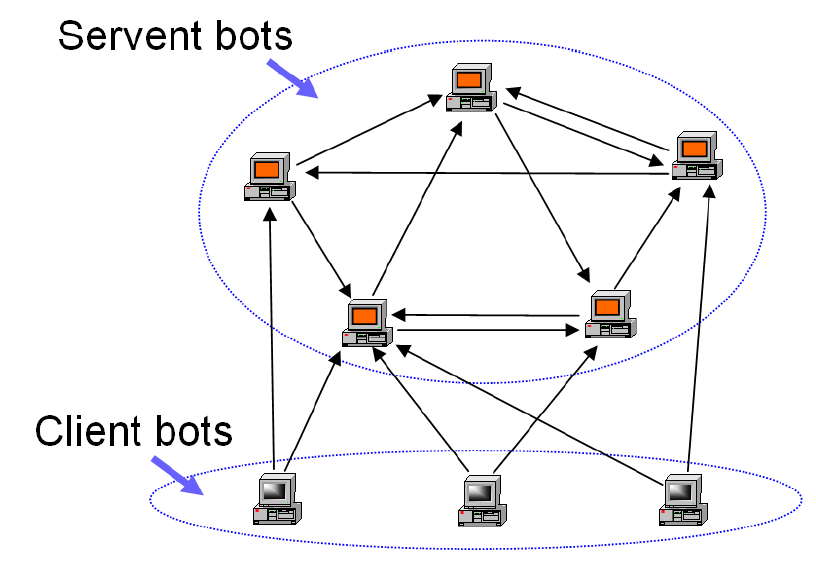
\includegraphics[scale=0.3]{hybrid}
\caption{Architecture d'un botnet hybride}
\end{figure}
\subsubsection{Utilisations}
Ils sont considérés comme le plus grand danger d'Internet. Pour les attaques DDoS ou les spams, aujourd'hui on sait qu'il y a beaucoup plus de spams envoyés que de mails légitimes. Les spams sont envoyés via des botnets. On a récemment découvert qu'un énorme botnet de frigos LG connectés (accessibles via les credentials par défauts) envoyait des emails de spams partout dans le monde. Il est possible de monitorer le botnet.\\
Les botnets servent aussi à récupérer des informations.
\begin{itemize}
\item Click fraud: cliquer en masse sur des pubs afin d'éliminer des campagnes de pub chez des concurrents qui payent leurs campagne au nombre de clic.
\item Le nombre de vues ou de likes peut également être utilisé via des botnets.
\item Cryptojacking: Les botnets peuvent être utilisés pour miner des cryptomonnaies.
\end{itemize}
\subsubsection{Communication au sein du botnet}
IRC était utilisé pour la communication entre les machines infectées et et C\&C. IRC permet à la fois de communiquer de façon multicast à tous les bots ou bien unicast à un seul bot. Mais vu que certaines entreprises n'ont pas à utiliser des protocoles de messagerie, le blocage d'IRC permet alors de bloquer le fonctionnement du bot (ex: Kaiten, Agobot).\\\\
Aujourd'hui on utilise majoritairement HTTP car toutes les entreprises l'utilisent et il est compliqué de le bloquer (ex: Zeus)
En 2019, 95\% des machines infectées sont sont des Linux et 5\% des Windows. Pourquoi? Car les objets connectés utilisent souvent un Linux et sont facile à infecter. Le moteur de recherche Shodan permet de chercher des machines IOT à infecter. Mirai est aujourd'hui le botnet qui a fait le plus de dégats, il infectait les objets connectés et majoritairement les caméras. \href{https://fr.wikipedia.org/wiki/Mirai_(logiciel_malveillant)}{Wikipedia: Mirai}
\begin{figure}[H]
\centering
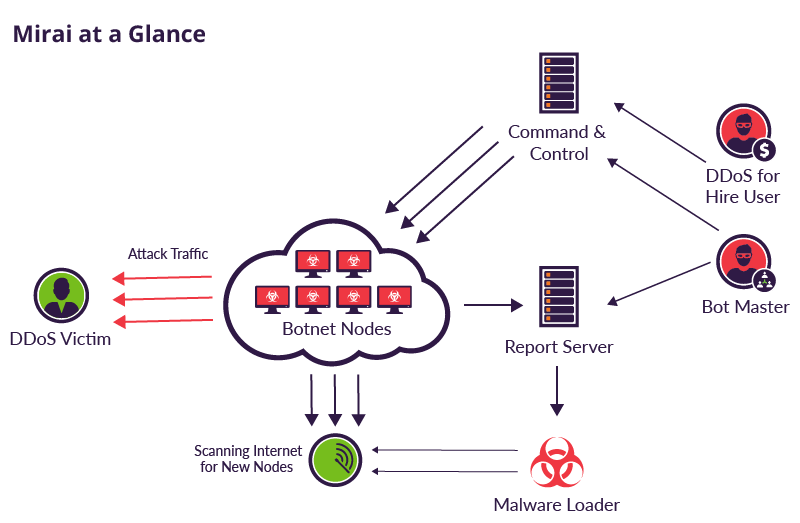
\includegraphics[scale=0.3]{mirai}
\caption{Architecture du botnet Mirai}
\end{figure}
\subsection{Botdloud}
\begin{itemize}
\item Il est possible d'utiliser des instances cloud afin de créer des botnets.
\item Disponible sur demande: élastique.
\item Légal, car il n'est pas illégal de louer des machines sur le cloud.
\item Le nom de l'hébergeur cloud permet aux cible de faire confiance. Si c'est AWS, la cible aura confiance en Amazon.
\item Les grands groupes de cloud ne donneront pas leurs logs facilement, donc compliqué à tracer les botnets.
il est possible de faire plein d'attaques grâce au cloud, et le service cloud n'envoie aucun avertissement.
\item Afin de créer un botcloud, les hackers vont utiliser un batch de cartes de crédit achetées sur le dark web afin de ne pas laisser de traces de leurs coordonnées bancaires. Il a été possible de craquer une clé wifi WPA en 6 minutes pour \$2. En lançant un DDoS qui dure 21 jours, AWS n'a envoyé aucun avertissement.
\end{itemize}

\subsubsection{Informations générales}
\begin{itemize}
\item CyberBunker: CyberBunker a servi d'hébergeur pour The Pirate Bay et l'un des nombreux miroirs de WikiLeaks. CyberBunker a également été accusé d'héberger des spammeurs, des serveurs de commande et de contrôle de botnet, des logiciels malveillants et des escroqueries en ligne.

\item IP stresser: outil utilisé pour tester la robustesse d'un réseau en envoyant plein de requêtes et vérifiant si le site les handle correctement. Les booters utilisent cette technique pour attaquer. Il est possible de générer des vraies cartes bancaires avec des générateurs puis de créer des instances cloud gratuites (souvent proposé chez tous les clouds GCP, AWS, Azure etc) puis de créer un botnet et le monitorer.
\item Les organisations de cloud vérifient ce qui entre dans les machines mais pas réellement ce qui en sort. Shodan + GHDB permet d'effectuer des actions sur les objets trouvés sur Shodan.
\end{itemize}

\end{document}